\documentclass[a0,landscape,pdftex]{a0poster}

\usepackage{amsthm,amsmath,amssymb,amsfonts,graphicx,algorithm,algorithmic}
\usepackage[scaled=1.1]{helvet}
\usepackage{postercols2}
\usepackage{flowfram}
\usepackage{color}
\usepackage{lipsum}
\usepackage{rotating}
\usepackage{subcaption}
\usepackage{booktabs}
\usepackage{multirow}
\usepackage{multicol}
\usepackage{paper_commands}


\setlength{\flowframesep}{.2in}
\setlength\parindent{0pt}
\setlength{\vcolumnsep}{.5in}
\setlength{\columnsep}{\vcolumnsep}

\Ncolumntop{static}{2}{3in}
\setstaticframe{1}{label={title}}

\newlength\offset
\setlength{\offset}{18.5in}
\addtolength{\offset}{\vcolumnsep}
\computeflowframearea{2}
\addtolength{\ffareaheight}{-\offset}
%\setflowframe{2}{height=\ffareaheight}
\addtolength{\ffareaheight}{\vcolumnsep}
%\newstaticframe{\ffareawidth}{18.5in}{\ffareax}{\ffareaheight}[figures]
\setstaticframe{20}{clear}

%this puts borders on the frames
%\setallflowframes{border=plain}
%\setallstaticframes{border=plain}

\title{Disentangling and Integrating Relational and Sensory Information in Transformer Architectures}
%\author{}
\date{}


\begin{document}

\begin{staticcontents*}{title}
\maketitle
\end{staticcontents*}
\thispagestyle{empty}

\Large

\section*{Relational games}

\begin{minipage}{55cm}




\begin{center}
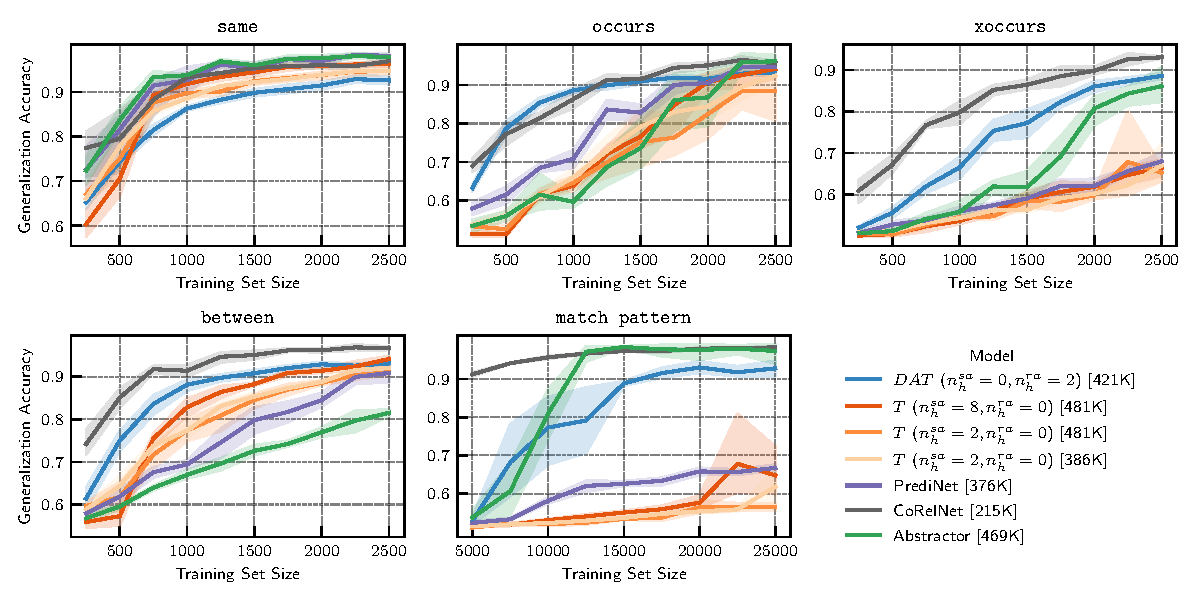
\includegraphics[width=0.95\textwidth]{../figs/experiments/relgames/relgames_learning_curves_baseline_comparisons.pdf}
\end{center}
{\rm Figure 1. Learning curves on relational games, comparing \textit{DAT} against multiple Transformer baselines of varying sizes and architectural hyperparameters (e.g., \# of heads).}
\vskip2cm


\section*{Mathematics processing}




% maybe pick one of the two 
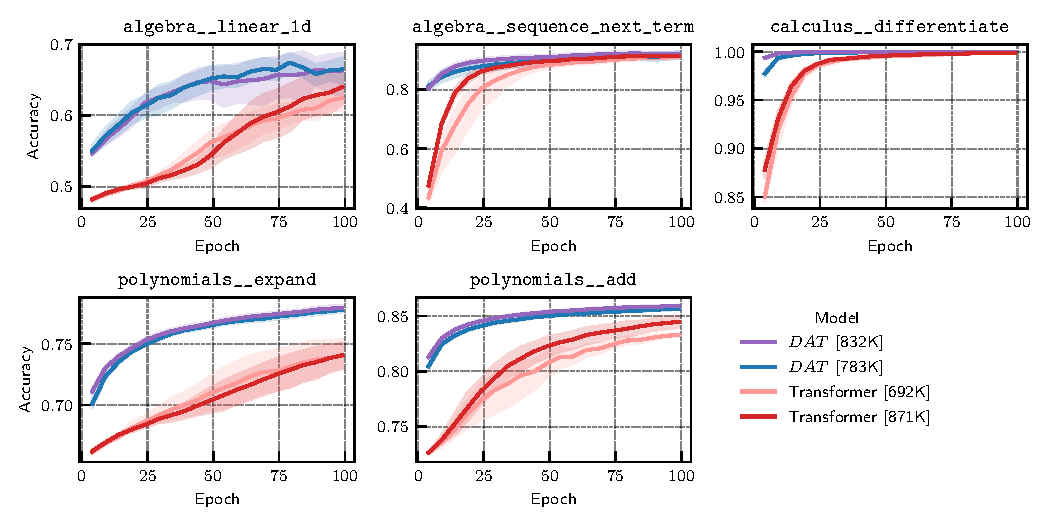
\includegraphics[width=0.95\textwidth]{../figs/experiments/math/math_training_curves_interpolation.pdf}

{\rm Figure 2. Validation accuracy over the course of training for seq2seq mathematical problem-solving;
number of parameters shown in brackets.}
\end{minipage}


\begin{minipage}{55cm}

\section*{Language modeling at larger scale}

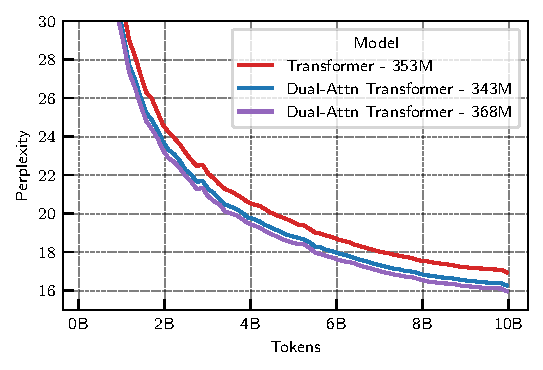
\includegraphics[width=.50\textwidth]{../figs/experiments/fineweb/350M_scale_lm.pdf}
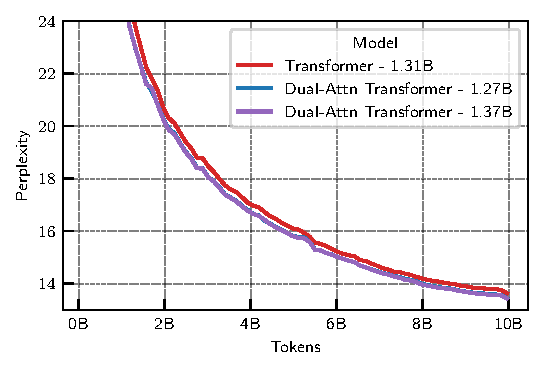
\includegraphics[width=.50\textwidth]{../figs/experiments/fineweb/1_3B_scale_lm.pdf}

{Figure 3. Perplexity for language modeling with the Fineweb dataset, for different size models. The $x$-axis indicates the number of tokens and the $y$-axis is the validation perplexity. Left: Each model has 24 layers; Transformer has 16 sensory heads; DAT models have 8 sensory heads and 8 relational heads; relational heads have 32-dimensional relations. Right: Each model has 24 layers; Transformer has 32 sensory heads; DAT models have 16 sensory heads and 16 relational heads; relational heads have 64-dimensional relations.}

\vskip3cm
\begin{tabular}{lll}
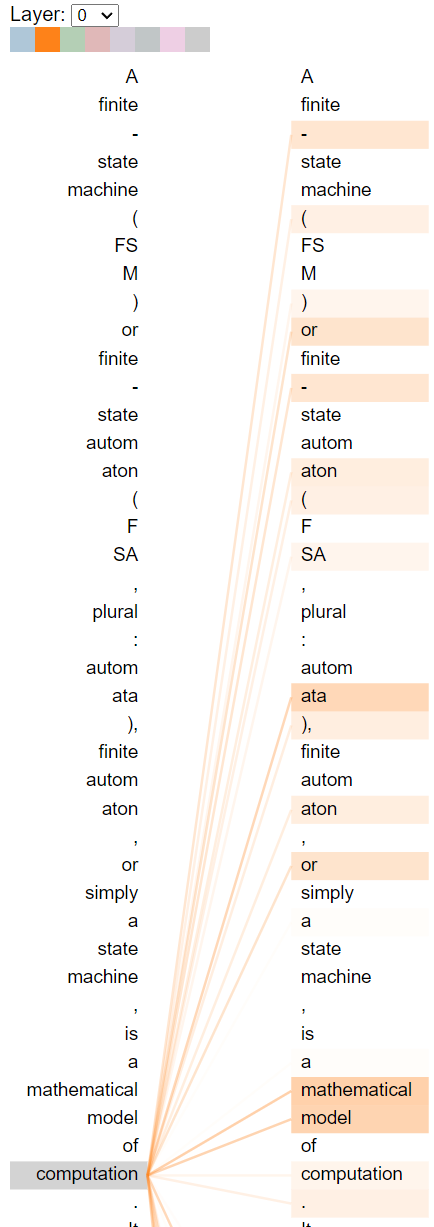
\includegraphics[width=.20\textwidth]{attn1} &
\qquad \raisebox{-3.2cm}{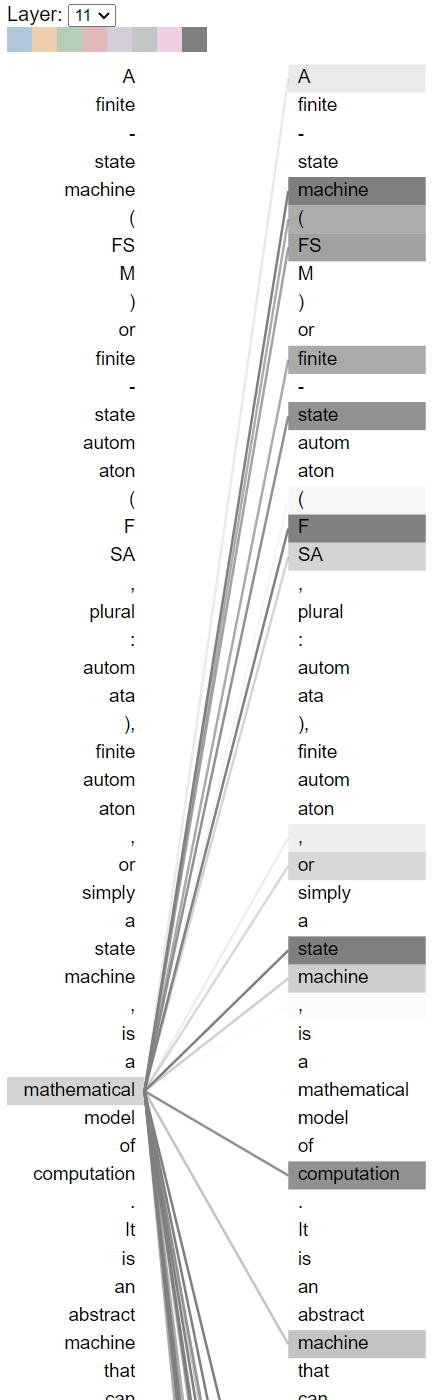
\includegraphics[width=.20\textwidth]{attn2}} &
\qquad \raisebox{28cm}{\begin{minipage}{25cm} Figure 4. Diagrams showing attention scores used by relational heads in two layers of a \sl{DAT} model trained on the Fineweb data. \end{minipage}}
\end{tabular}

\vskip2cm
\end{minipage}


\end{document}
